\section{Design}

\subsection{System-level design}
The complete system will consist of energy harvesting source, energy storage for times when harvested energy is not available, AC/DC and DC/DC converters for maintaining required voltage levels in different blocks of system, accelerometer for measuring the accleration in tyre and radio/microcontroller module for transmitting data from acceleromoter. Figure \ref{fiq:system_block_diagram} shows the power and data flow between subsections of system. 


\begin{figure}[htb]
\begin{center}
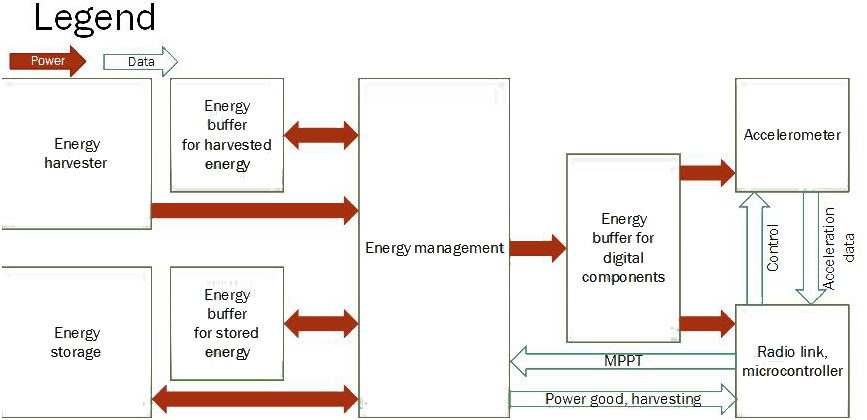
\includegraphics[height=6cm]{images/own_dwg/system_block_diagram.jpg}
\end{center}
\caption{\label{fiq:system_block_diagram} Block diagram of complete system.}
\label{liitekuva}
\end{figure}

Energy harvester can be any suitable source for electrical energy. Energy management section rectifies AC voltage and buffers the rectified voltage on a capacitor. The energy storage can be a supercapacitor or rechargeable battery. Both of these storage technologies can benefit from having a low equivalent series resistance (ESR) capacitor in parallel to supply any sudden peak currents. Energy management circuitry chooses whether to use harvested energy or stored energy and regulates the energy to voltage level compatible with the system. Digital components require their own local power buffer capacitors to supply high-frequency currents required by megahertz clocks onboard these circuits.

Microcontroller is used to manage the application layer of system. For example the microcontroller can send status updates over radiolink more often if there is harvested energy available and reduce system power consumption when system is running on stored energy.

Next section presents details of expected power consumption and duty cycles for various components. A few components are selected to provide examples of suitable system power.

\subsection{Power requirements of a system} \label{sect:power_requirement}
The sensor system will be in three distinct states. One is sleeping, conserving power as much as possible while car is not moving.
Second state is measuring, when the radio connection is off but electronics are active and gathering data.
Third state is transmitting, when the data is relayed to drive computer in car.

Energy and power consumption are estimated by reviewing a few suitable components and their power requirements. 
Energy management is handled by a specialised integrated circuit (IC), for example LTC3331 \cite{Technology}.

Communication is handled by a Bluetooth-low energy (BLE) module, which contains a general-purpose microcontroller for application flow control.
We use BLE113 \cite{Bluegiga2013} as an example of such module.

Finally there is an accelerometer which is used for gathering data out of the system, ADXL375 \cite{ADXLDatasheet} is used as an example. ADXL is a low-power digital accelerometer with dynamic range of 200g. Table \ref{power_consumption_table}  summarises the estimated power requirement of each subsection of system. System level voltage is selected to be 2.5 V, as that is lowest voltage which LTC3331 can supply and allows all devices to function. Lowest possible voltage is selected to reduce the power draw.

\begin{table}[htb]
\caption{\label{power_consumption_table} Current and power consumption of system at different activity levels.}
\begin{center}
\fbox{
\begin{tabular}{l l r r}
\textbf{Device}		& \textbf{Sleep} 	& \textbf{Monitoring}	& \textbf{Communicating}\\ \hline
LTC3331			& 0.2 $\mu A$		& 80 $\mu A$ 		& 16 250 $\mu A$ 		\\ \hline
BLE113			& 0.9 $\mu A$ 		& 275 $\mu A$ 		& 26 000 $\mu A$	\\ \hline 
ADXL375			& 0.1 $\mu A$ 		& 140 $\mu A$ 		& 140 $\mu A$		\\ \hline \hline
\textbf{Total power}	& 3   $\mu W$		& 1 200 $\mu W$		& 110 000 $\mu W$	
\end{tabular}
}
\end{center}
\end{table}

Current consumption levels for BLE113 and ADXL375 are taken from the datasheets of the components. Battery manager power draw is estimated by calculating required power to supply the rest of the circuit at 80 \% efficiency. Power consumption is calculated from current draw with assumption that system voltage will be constant $2.5 V$.

Power consumption grows by orders of magnitude when the activity is stepped up to the next level. Therefore it is important to keep the system in sleep whenever possible, for example when the car is parked and wake up only periodically to check if movement has started. Monitoring starts once car is moving, and device will send brief pulses over the radio link when necessary.

When the power consumption is compared to values achieved in previous studies of energy harvesting, it can be seen that sleep current can be compensated by a reasonable harvester design. Powering constant monitoring would be a greater challenge, but with realm of feasibility. Providing power for continuous radio transmissions is not feasible even with current state-of-the-art harvester designs. 

Next sections detail designs and preliminary analysis of electromagnetic generator designs. The initial designs are then evaluated based on their ability to supply required power levels to circuitry.

\subsection{Electromagnetic harvester design}
The focus for this section is in designing a macro-scale linear generator for harvesting energy. The previous work in area is presented in the first subsection, analytical model for harvester is presented in second subsection. Third subsection presents simulation model which uses FEM analysis of magnetic properties of generator as well as preliminary experimental validation of model and concept. Final subsection details the completed design of harvester.

\subsubsection{Basics of electromagnetical vibration harvester}
Electromagnetic harvesters utilise vibration to move a magnet inside a coil. The movement of a magnet causes a changing magnetic field, which gets coupled to a coil. The coil opposes the change in magnetic field by inducing electrical current in the device. A device could be built with a spring-loaded magnet to balance out the static acceleration of a tyre, an added benefit to spring loaded mechanism would be the utilisation of resonant frequency of the spring-mass system: as the system gets a shock, some of the energy would be in correct frequency range to make the magnet oscillate inside coil allowing generation of energy until next shock. The coil will also function as a damper to system, so no extra damping is required. Modern neodymium magnets do not lose their magnetization by vibration, so long magnet can be reliable for a long time period. 

A theoretical design of linear generator (LG) was made. Most common generator designs use a rotating magnet inside coils to generate alternating current. As the mechanical apparatus for converting the linear accelerations inside the tyre to rotational movement would add to complexity and cost of the tyre, generator is designed to use the linear motion as the power source.

Basic principle of operation of LG is similar to traditional rotational generator. A moving magnet creates alternating magnetic field which is coupled to coiled conductors. The conductors oppose this change of magnetic field by inducing an electrical current across their ends. The design can have multiple phases and poles, where phases refer to parallelly connected coils and poles refer to serially connected coils. Multiple phase designs can have lower resistive losses in wiring, as the resistive losses are propotional to square of the current. However paralleling phases requires separate rectification for each phase, which leads to increased rectification losses. Adding poles to design increases the output voltage and frequency, but having a small airgap between the coils and magnets becomes critical to maintain efficiency of the generator \cite{Cheng2008}. 

Energy harvester designs sometimes use several poles to increase the frequency of the power output. This increased frequency allows to use smaller energy storage components such as capacitors to keep the device powered until next cycle. The characteristics of the tyre make this point irrelevant, as energy is available once per revolution of the tire when generator contacts the ground and when the contact ends. Any energy storage device has to maintain power until the next cycle, and no increase of the frequency while generator is in contact can alleviate that. Therefore number of poles is minimized to reduce complexity. Pole number is selected as two, so there is one negative and one positive pole. Mechanical design can utilise resonant vibration to function as energy storage device instead of electrical or electronic storage.

First design decision was whether to use a moving magnet or moving coil type of a design. Moving coil designs tend to have lighter moving parts which is a very important feature in high-power designs where mass of the generator is large. On the other hand, moving coils require flying leads  \cite{Jacob2011},  which is a long-term reliability concern  \cite{Boldea1999}.  Boldea and Nasar \cite[p. 203]{Boldea1999a} conclude that moving coil designs aren't practically interesting, so the design is focused on moving magnet generator. 

A rough model for designing initial prototypes was done previously by Elmes \cite{Elmes2005}. As the work verified the model experimentally and found the model to be reasonably accurate, it was adapted to form basis of linear generator model. The model can account for most of the key design parameters. 

There are two different approaches to generator structure. One is magnets inside, and coils on the outer rim of the generator. Other is to use ring magnets on the outer rim and have the coils on the inside. Both methods have their advantages: Having magnets on the outside allows larger and therefore stronger magnets and creates horizontal support for the magnets as they move along the shaft. Having coils on the outside increases wiring radius which results in greater power if other parameters are held equal. In-depth study of both concepts is done to select optimal structure for generator. 

The height of the generator is constrained at 45 mm to avoid contact between tyre rim and generator. Initially the height of the generator was selected to be 35-40 mm to leave some margin while still being as tall as possible. Lower weight is desirable to avoid unbalancing the tyre, but there is no specific absolute maximum mass for the device. 

A method to counter the centripetal acceleration is needed to keep the magnet on the centre of the generator. Ideally, such method would always balance the magnet in the middle of generator against any external constant force, but active control is not achievable without adding to complexity and power consumption of the generator itself. Passive negative feedback method has to be used instead. 

Springs are often chosen to balance the magnets, but as the centripetal acceleration grows exponentially with the speed of the car, any linear spring would be usable only for very limited range of speeds. Non-linear conical springs which have the added benefit of compressing into very small height are available.

Another approach would be to use two additional magnets fixed to top and bottom of the generator in repulsive configuration. Force between magnets is inversely propotional to fourth power of the distance \cite{Amrani2015}, which leads to a strong negative feedback on the position of the magnet. Tornincasa et al. \cite{Tornincasa2012} proposed one such design, shown in figure \ref{lgm}.

\begin{figure}[htb]
\begin{center}
\includegraphics[height=4cm]{images/own_dwg/lgm}
\end{center}
\caption{A magnetically balanced linear generator by Tornincasa et al. \cite{Tornincasa2012}}.
\label{lgm}
\end{figure}

Magnetic floating is an attaractive solution, as magnets can be thin and they do not wear out with aging. On the other hand, any imbalance in the magnets result in torgue which causes increased friction. \ref{fig:lg_torgue} This issue is further aggravated in designs where shape of the generator shaft is not a smooth cylinder. Therefore the design should have reasonably smooth and low-friction material on the inner shaft to minimize losses.

\begin{figure}[htb]
\begin{center}
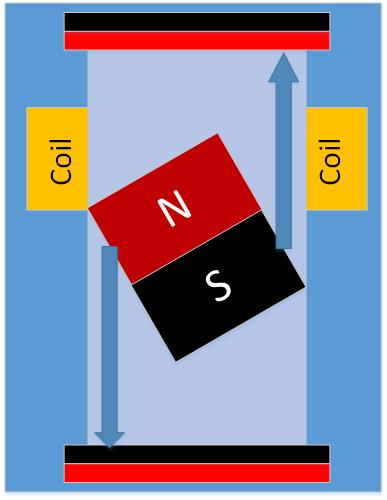
\includegraphics[height=6cm]{images/own_dwg/generator_torgue}
\end{center}
\caption{Angle in magnet causes torgue which results in increased friction}.
\label{fig:lg_torgue}
\end{figure}

\subsubsection{Analytical model of electromagnetical vibration harvester}
A common starting point for analysis of linear generator is to model the mechanical domain as Mass-Spring-Dampener system decipted in figure \ref{MSD}. A mass "floats" in system, a spring balances the mass towards centre and a damper represents frictional forces opposing any movement of mass. 

\begin{figure}[htb]
\begin{center}
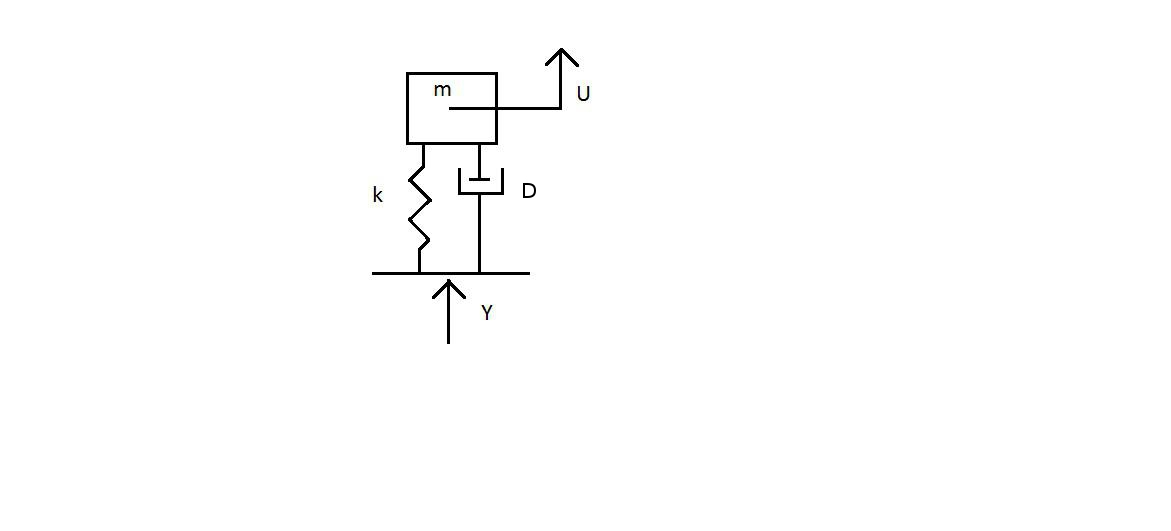
\includegraphics[height=6cm]{images/own_dwg/MSD.jpg}
\end{center}
\caption{\label{MSD} Mass-spring-damper system.}
\end{figure}

Input Y is the force applied to the base of system, output U is the position of mass block relative to "zero". Zero is usually set to point where mass settles when no input, including gravity, is applied to system. Paramters m, D, and k are mass, damping constant and spring constant of system, respectively. Input-output-equation in time domain can be written as: 

\begin{equation}\label{eq:MSD_basic}
  m * \ddot{U}(t) + D * \dot{U}(t) + k * U(t) = Y(t). 
\end{equation}

As the force $ Y(t) $ is defined as $ Y(t) = m*a(t) $, and the acceleration $ a(t)$ can be considered constant regardless of any reasonable mass $ m $ of system, equation \eqref{eq:MSD_basic} can be written as:

\begin{equation}\label{eq:MSD_acceleration}
 \ddot{U}(t) + \frac{D * \dot{U}(t)}{m} + \frac{k * U(t)}{m} = a(t). 
\end{equation}

This form is convenient for analysis, as the acceleration measurements from previous research are available and they represent real-world values. Mass m can be considered constant, as the system does not exchange matter with surrounding environment. As magnetic suspension was selected, the paramter k cannot be considered as a constant, but rather a function of mass position $k(U)$. Centripetal force can be considered as a constant DC-component of function $Y(t)$, and is not included in analysis of function $k(U)$. According to D. Amrani \cite{Amrani2015} force between two magnets can be approximated as

\begin{equation}\label{eq:magnetic_force}
  F(x) = \frac{3 \mu_0 m_1 m_2}{2 \pi} * \frac{1}{x^4},
\end{equation}

where $F(x)$ is force as a function of distance x between magnets, $\mu_0$ is the permeability of vacuum, $ m_1 $ and $ m_2 $ are magnetic dipole moments of magnets under examination. This equation is only valid when x >> h, where h is thickness of the magnet. As two magnets are used to suspend the rotor magnet, total force acting on mass becomes 

\begin{equation}\label{eq:magnetic_force_middle}
  F(x) = \frac{3 \mu_0 m_r m_l}{2 \pi} * \frac{1}{(x_0+x)^4} - \frac{3 \mu_0 m_r m_u}{2 \pi} * \frac{1}{(x_0-x)^4},
\end{equation}

where $m_l, m_u, m_r$ are magnetic dipole moments of lower suspending magnet, upper suspending magnet, and rotor magnet. $x_0$ is the distance to middle point of generator and $x$ is the displacement of rotor magnet from aforementioned middle point, positive direction being upwards. Figure \ref{fig:lg} shows the system.

\begin{figure}[htb]
\begin{center}
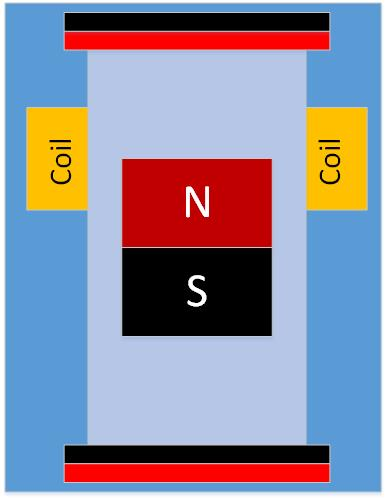
\includegraphics[height=6cm]{images/own_dwg/generator}
\end{center}
\caption{Linear generator with rotor magnet balanced by endstop magnets}.
\label{fig:lg}
\end{figure}

Regrettably, the expression \eqref{eq:magnetic_force_middle} is very inaccurate for magnets where diameter is large compared to thickness of magnet, and the problems are compounded when distance between magnets is small. Therefore final design should be optimized using measurement data or finite element analysis (FEA) for determining $k(U)$. 

Damping parameter $D$ is likevise a function electromagnetic force acting on magnet, friction between magnet and stator and pneumatic damping caused by compression of air in generator. Tornincasa et al. \cite{Tornincasa2012} divided this damping parameter into three distinct terms to account for these different physical phenomena in damping. Let us call them $D_{emf}, D_{friction},$ and $D_{air}$, respectively. $D_{emf}$ represents power extracted from the system into electrical current, it can be written as:

\begin{equation}\label{eq:d_emd}
  D_{emf} = BIlsin(\phi),
\end{equation}

where $B$ is magnetic field affecting coil (presumed constant), $I$ is current through wire depending on load and generator properties, $l$ is total length of wire in coil and $\phi$ is angle between coil and magnetic field, presumed to be 90 \degree. Assuming the load impedance is the complex conjugate of coil impedance for maximum power harvesting, we can substitute the $I$ with equations \eqref{eq:emf} and \eqref{eq:gen_simple_current}, which results in: 

\begin{equation}
  D_{emf} = B \frac{\varepsilon}{2*Re(Z_{generator})} l sin(90 \degree),
\end{equation}

where $Z_{generator}$ is the impedance of generator. As the load impedance is complex conjugate of generator impedance, their series connection has only real (purely resistive) component. This assumption fails on real-world application with non-linear rectification and DC/DC conversion, but it can be used as a basis for analytical examination of the generator. As $\varepsilon$ can be substituted with \eqref{eq:emf}, we obtain:

\begin{equation}\label{eq:d_emf_with_epsilon}
  D_{emf} = B \frac{-N \frac{d \Phi_{B}}{d t}}{2*Re(Z_{generator})} l sin(90 \degree),
\end{equation}

The relationship between $N \Phi_{B}$ and $Re(Z_{generator})$ can be further studied by writing 

\begin{equation}\label{eq:phiB_substitution}
  \Phi_{B} = \iint_{\Sigma (t)} B(r, t) \,dA,
\end{equation}

 where $ \iint_{\Sigma (t)} $ signifies possibility of loop area changing over time and $\,dA$ is element of surface area. If we assume the coil to be a perfect tightly wound circle which does not deform over time, we can write the relationship between number of turns in coil, area of coil, and resistance of coil as:

\begin{equation}\label{eq:nA_R}
  R = N 2\pi A \rho_{wire},
\end{equation}

where $\rho_{wire}$ is resistivity of coil wire. Substituting \eqref{eq:nA_R} and \eqref{eq:phiB_substitution} into \eqref{eq:d_emf_with_epsilon} we finally obtain reasonably accurate expression for $D_{emf}$ which accounts for all the design parameters affecting it:
\begin{equation}\label{eq:d_emf_complete}
  D_{emf} = B \frac{-N \frac{d [\iint B(r, t) \,dA]}{d t}}{2*N 2\pi A \rho_{wire}} l sin(90 \degree).
\end{equation}

A few observations can be made from this equation: first, the magnetic field strength $B$ and it's derivate in respect to time increase the $D_{emf}$ which signifies the electrically extracted useful power. Therefore it makes sense to use as strong magnets as possible, as long as other parameters aren't adversely affected. Second, both the number of turns and the loop area are as multipliers and divisors, which means  they should be optimized to find best applicable values. Third, resistivity of wire limits power that can be extracted, so intuition would lead to minimizing wire resistance. In practise the wire resistivity can be decreased by increasing wire diameter, which in turn leads to lesser number of turns in same volume and mass of coil. Therefore, also wire diameter and material should be optimized to find desirable compromise in generator design. 

Next we examine $D_{friction}$ in detail. Friction is modelled as Couloumb fricion:
\begin{equation}\label{eq:couloumb_friction}
  F_s = \mu_sN,
  F_k = \mu_kN,
\end{equation}

where $F_s $ and $ F_k $ are static and kinetic friction forces opposing movement, $\mu_s$ and $\mu_k$ are friction coefficients in static and kinetic situations and $N$ is normal force along X- or Y- axis. Normal forces are estimated by using existing acceleration data and calculated mass of magnet. Coefficients of friction are looked up from supplier of stator material. Transfer between static and kinetic models is assumed to be a step, if velocity of magnet is 0 along Z-axis, $\mu_s$ is used, $\mu_k$ othervise.

Finally, there is pneumatic damping of the system, $D_{air}$. In a closed tube, the central magnet can be thought as a piston dividing generator into two chambers. If there is insignificant airflow between chambers, any force caused by pressure deltas between chambers act as a spring. However, some airflow is to be expected due to clearance between magnet and stator. Tornincasa et al. \cite{Tornincasa2012} modelled this effect by adding a virtual centrepoint for pneumatic spring, this centre moves through a virtual damper which models the airflow between chambers. End result is that pneumatic spring takes some energy from movement, and this energy stored into pneumatic spring is dissipated as the centre moves until potential energy stored in the spring is zero. 

The force from pressure differential is:

\begin{equation}
  F_{\delta p} = \frac{\pi d^2}{4}(p_{lower}-p_{upper}),
\end{equation}

where $d$ is diameter of magnet and $p_{lower}-p_{upper}$ are pressures in chambers. Pressures can be estimated from ideal gas law:

\begin{equation}
  pV = NRT
\end{equation}
where $p$ is pressure, $V$ is volume, $N$ is amount, $R$ is ideal gas constant and $T$ is temperature. Temperature is assumed to be constant. Initial pressure is assumed to be same as tyre pressure and magnet is assumed to be exactly in midpoint at start. Change of volume can be calculated from change of height caused by movement of the magnet. 

Mass flow between sections can be estimated with equation given by Fox et al. \cite{Fox2008}:

\begin{equation}
  \dot{m}_{1 \rightarrow 2} = \frac{\rho \pi d {\delta_r}^3}{12\mu h}(p_1-p_2),
\end{equation}

where $\rho$ is air density, $\delta_r$ is radial clearance, $\mu$ is dynamic viscosity and $h$ is the height of magnet. \cite{Tornincasa2012}

There is also frictional dissipative force as the air passes along the edges of the cylinder. This frictional force has magnitude of: 

\begin{equation}
  F = \mu * \rho * \frac{\pi d h \dot{z}}{\delta} \cite{Medhat2008}. 
\end{equation}

Analytical expressions for the equations governing the mechanical movement of magnet inside generator have now been identified. Some of the non-linear functions are hard to solve analytically, therefore experimental or FEA methods should be used for creating approximations for these functions.

The analytical effect of these parameters is summarized in table \ref{parameters_of_lg}

\begin{table}[htb]
\caption{\label{parameters_of_lg} Effect of parameters of generator}
\begin{center}
\fbox{
\begin{tabular}{l l l}
\textbf{Parameter}          & \textbf{Increasing} 		& \textbf{Decreasing}	\\ \hline
\(\displaystyle N_{turns} \)& Higher voltage		& Smaller size, less wiring resistance 		\\ \hline
\(\displaystyle N_{pole} \) & Increased frequency		& Decreased frequency	\\ \hline
\(\displaystyle l_{pole} \) & More space for wiring 	& Higher voltage, smaller size	\\ \hline
\(\displaystyle A_{loop} \) & More power			& Smaller length of wiring 	\\ \hline
B                           & Increased power 	        & Smaller magnets 		\\ \hline
\(\displaystyle r_{wire}\)  & Decreased wiring resistance 	& More turns in same space 	\\ \hline
\(\displaystyle \delta_{r} \) & Stronger side walls		& Incresed efficiency 
\end{tabular}
}
\end{center}
\end{table}


\subsubsection{Experimental and FEA modeling of electromagnetic harvester}
As some parameters of the harvester are difficult to solve analytically, these parameters are solved using experimental and FEA methods. First one of these difficult interactions is the magnetic force between rotor magnet and balancing magnets. A magnetics FEA software FEMM \cite{Meeker2013} was used to create an axisymmetric model of magnets in generator. Figure \ref{femm_forces} shows the used model. Model has two biasing magnets made of N40-neodymium alloy configured to repel an identical rotor magnet. Magnets have height of 2.5 mm and diameter of 11 mm, walls of generator are modelled as air. Generator has total height of 25 mm, leaving rotor magnet 17.5 mm room for movement inside generator.

Weighted stress tensor integration over rotor magnet volume as implemented by FEMM was used to determine FEA value for net magnetic force acting on rotor magnet. A LUA script was used to move the rotor magnet from bottom of the generator to top in 0.1 mm increments and values obtained from analysis were exported as CSV data for plotting in a spreadsheet software as well as to create a lookup-table for MATLAB/SIMULINK simulation. Figure \ref{femm_forces} shows the force on magnet, positive force meaning force towards the upper magnet and zero height being at the bottom of cylinder. For reference the centrifugal force acting on magnet was also calculated at various speeds, assuming weight of the magnet is 1,67 g and radius to bottom of generator is 275 mm.

\begin{figure}[htb]
  \begin{center}
  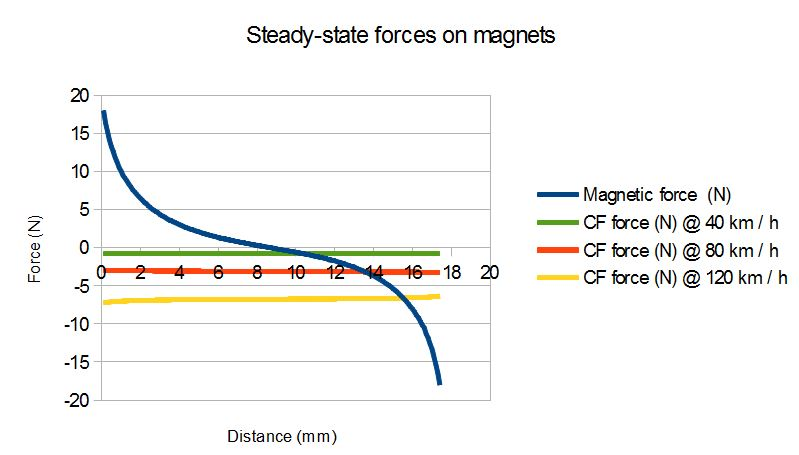
\includegraphics[height=6cm]{images/own_dwg/femm_fvsd_dualmagnet.jpg}
  \end{center}
  \caption{\label{femm_forces} Steady-state forces acting on magnet}
\end{figure}

It can be seen that net force on rotor magnet is dominated by the magnetic forces at lower speeds. Centrifugal force on magnet becomes significant at higher speeds, but even at 120 km/h speed the rotor magnet will stay clear of the bottom. Second use for this FEA analysis is to create look-up table for flux linkage into coils of generator. The methodology was similar to determining forces affecting the rotor magnet: a LUA script was ran to sweep possible magnet positions, and look-up table of flux linkage into coils was created. For the purposes of analysis, difference of flux linkage was calculated between each point. The change of flux linkage is a very important parameter, as the power generated is proportional to $\frac{d \Phi_{B}}{d t}$. 

\begin{figure}[htb]
\begin{center}
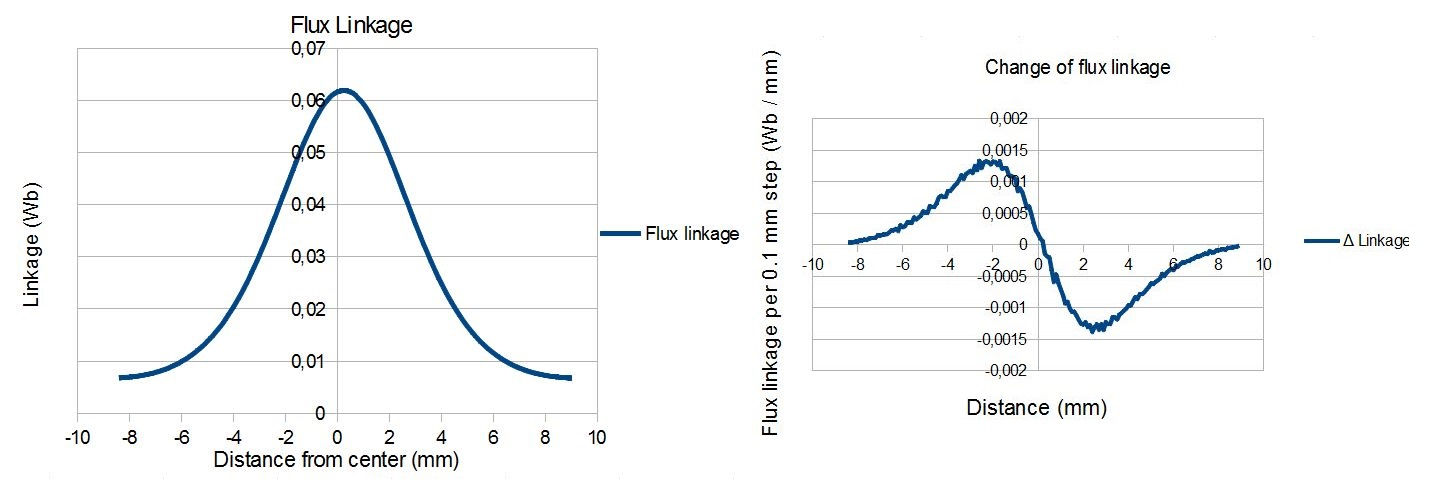
\includegraphics[height=6cm]{images/own_dwg/femm_flux_dualmagnet.jpg}
\end{center}
\caption{\label{fig:femm_linkage} Flux linkage and rate of change in 0.1 mm steps in generator.}
\end{figure}

Based on these results, a magnet moving at the speed of $0.1 mm / s $ would induce voltage of up to $1.5 mV$ in each winding of the coil. If we assume coil to have 100 turns, travel length of the magnet to be 1 mm, and frequency of magnet moving inside generator to be 10 Hz the peak voltage out of generator would be sufficient to power the circuitry and charge battery of sensor.

A prototype generator was built to test the concept feasibility and identify any practical issues in the generator construction. Generator was machined out of 21mm diameter nylon tubing with 12 mm inner diameter. A groove was machined on the outer diameter to hold the coiling in place. Inner diameter of the groove was 14 mm and height 3 mm. 0.1 mm diameter wire was used to build the coil. To determine the number of turns in coil, coil resistance was measured to determine the length of wire and number of turn was calculated using known length of loop turn and total length of wire. Coil resistance was 42 ohms as the resistance of wire is approximately 2.2 ohms / meter the total length is approximately 19 meters. As one loop has length of 44 mm, coil had roughly 400 turns. 

The prototype was connected on a  Brüel & Kjær shaker type 4905 and driven using  Brüel & Kjær power amplifier type 2707. Input signal was generated using NI-USB6218 DAQ and output was measured directly from leads of the generator. Vertical displacement of generator was limited to $7.5 mm$. Output signal was a sine wave with amplitude of \plusminus 5 volts, which was amplified by gain of 8 above frequencies of 30 Hz. At lower frequencies the gain was limited to stay within allowed displacement. Measured graphs are shown in figure \ref{fiq:lg_proto_results}.

\begin{figure}[h]
\begin{center}
  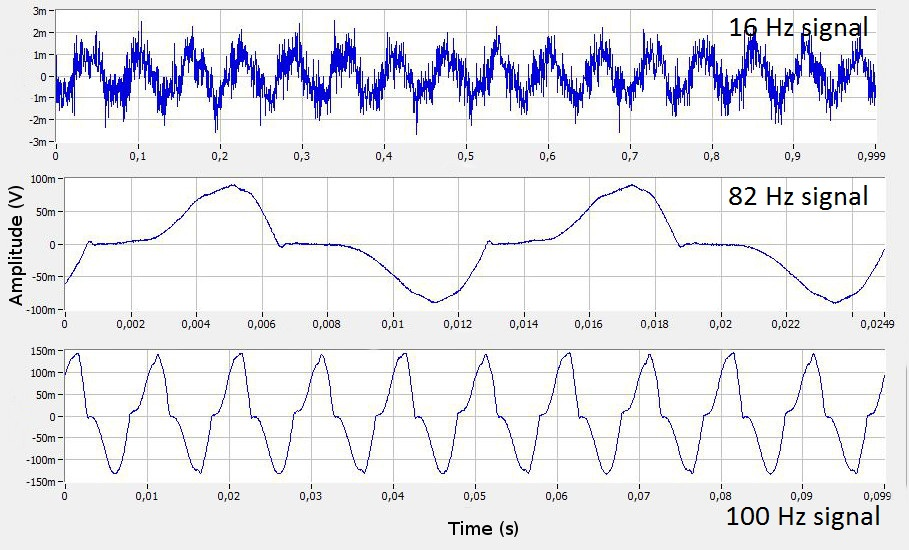
\includegraphics[height=8cm]{images/own_measurement/lg_proto.jpg}
  \end{center}
  \caption{\label{fiq:lg_proto_results} Measured open-loop voltage outputs at various frequencies}
\end{figure}

At low frequencies the magnets do not overcome friction and only measurement noise is present in signal. In addition to white noise in measurement there is a sine wave with amplitude of hew millivolts which correlates with the excitation signal. The measurement noise is insignificant when compared to signal generated my moving magnet. 

At low frequencies the magnet cannot overcome the friction and only noise is present in measeurement. Around 82 Hz the magnet could move inside shaft, producing peaks with roughly 100 $mV$ peaks. The magnet stops in between of the peaks which is seen as valleys of no voltage being produced. 

Peak voltages of roughly 150 mV were achieved at 100 Hz. The magnet is in almost constant motion, a brief stop can be seen when the magnet changes direction. 

While 150 mV is notably less than the few volts predicted by Simulink model, the basic operation principles was validated by quick experiment. The difference in output voltage is probably due to inprecise construction in prototype harvester. As the concept was proven, the design of generator was finalized. Next section details the exact construction of final electromagnetic generator. 

\subsubsection{Mechanical design of electromagnetic harvester}\label{sect:emh_design}
Few practical issues became evident during construction of prototype generator. Machining grooves to plastic tubes caused warping to tube, which prevented magnet from moving inside coils. Shallow grooves would not keep the coils in place, as wires being loose would fall off the groove. The tube did not offer any reasonable mount point for a printed circuit board. 

Issues with grooves were solved by selecting a tube with minimal wall thickness and using separators to contain the coil. A separate housing was designed to hold the tube and to offer mounting points for the circuit board. 

A layered design was made for the harvester. On the bottom is a solid square with 35 * 35 mm sides and holes for screws on corners. Next layer has a hole for the bottom magnet, third layer has hole for the tube. Tube has a spacer in middle to hold the coil below midpoint. Top half of harvester is symmetrical to bottom. 

\subsection{Piezoelectric harvester design}
\subsubsection{Basics of piezoelectric energy harvesting }
This section details experimental identification of properties of piezoelectric element to be used in harvester. A testbed with impactor providing excitation is used to generate experimental values for power output and voltage at various operating conditions for the piezo element.

Thunder(tm) piezos have been used in previous studies of piezoelectric harvesting and they have produced promising results \cite{Manla2009}, so they were selected as the piezoelectric element for this thesis.

Series of tests were ran to determine characteristics of piezoelectric power generation under impacts. Mossi et al \cite{Mossi} have produced a recommended test process for Thunder piezoelectric actuators shown in figure \ref{fiq:thunder_eval}.

\begin{figure}[htb]
  \begin{center}
  \includegraphics[height=6cm]{images/cited/mossi}
  \end{center}
  \caption{Recommended evaluation platform for Thunder piezos \cite{Mossi}.}
  \label{fiq:thunder_eval}
\end{figure}

This setup was replicated using a solenoid actuator as impact force generator, precision scale as load cell to measure impact force and oscilloscope to view output waveforms. An eraser was cut to shape to act as preload bellow to spread the impact over larger surface area of piezo, displacement was not measured. The test setup is shown in figure \ref{fiq:piezo_impact}. An electronics prototyping platform, "breadboard", was used to house test electronics including resistive ladder and Arduino to trigger the solenoid at adjustable duty cycles. Load force was controlled by setting the stroke length of solenoid shaft and fine tuned by adjusting voltage over solenoid. 

\begin{figure}[htb]
  \begin{center}
  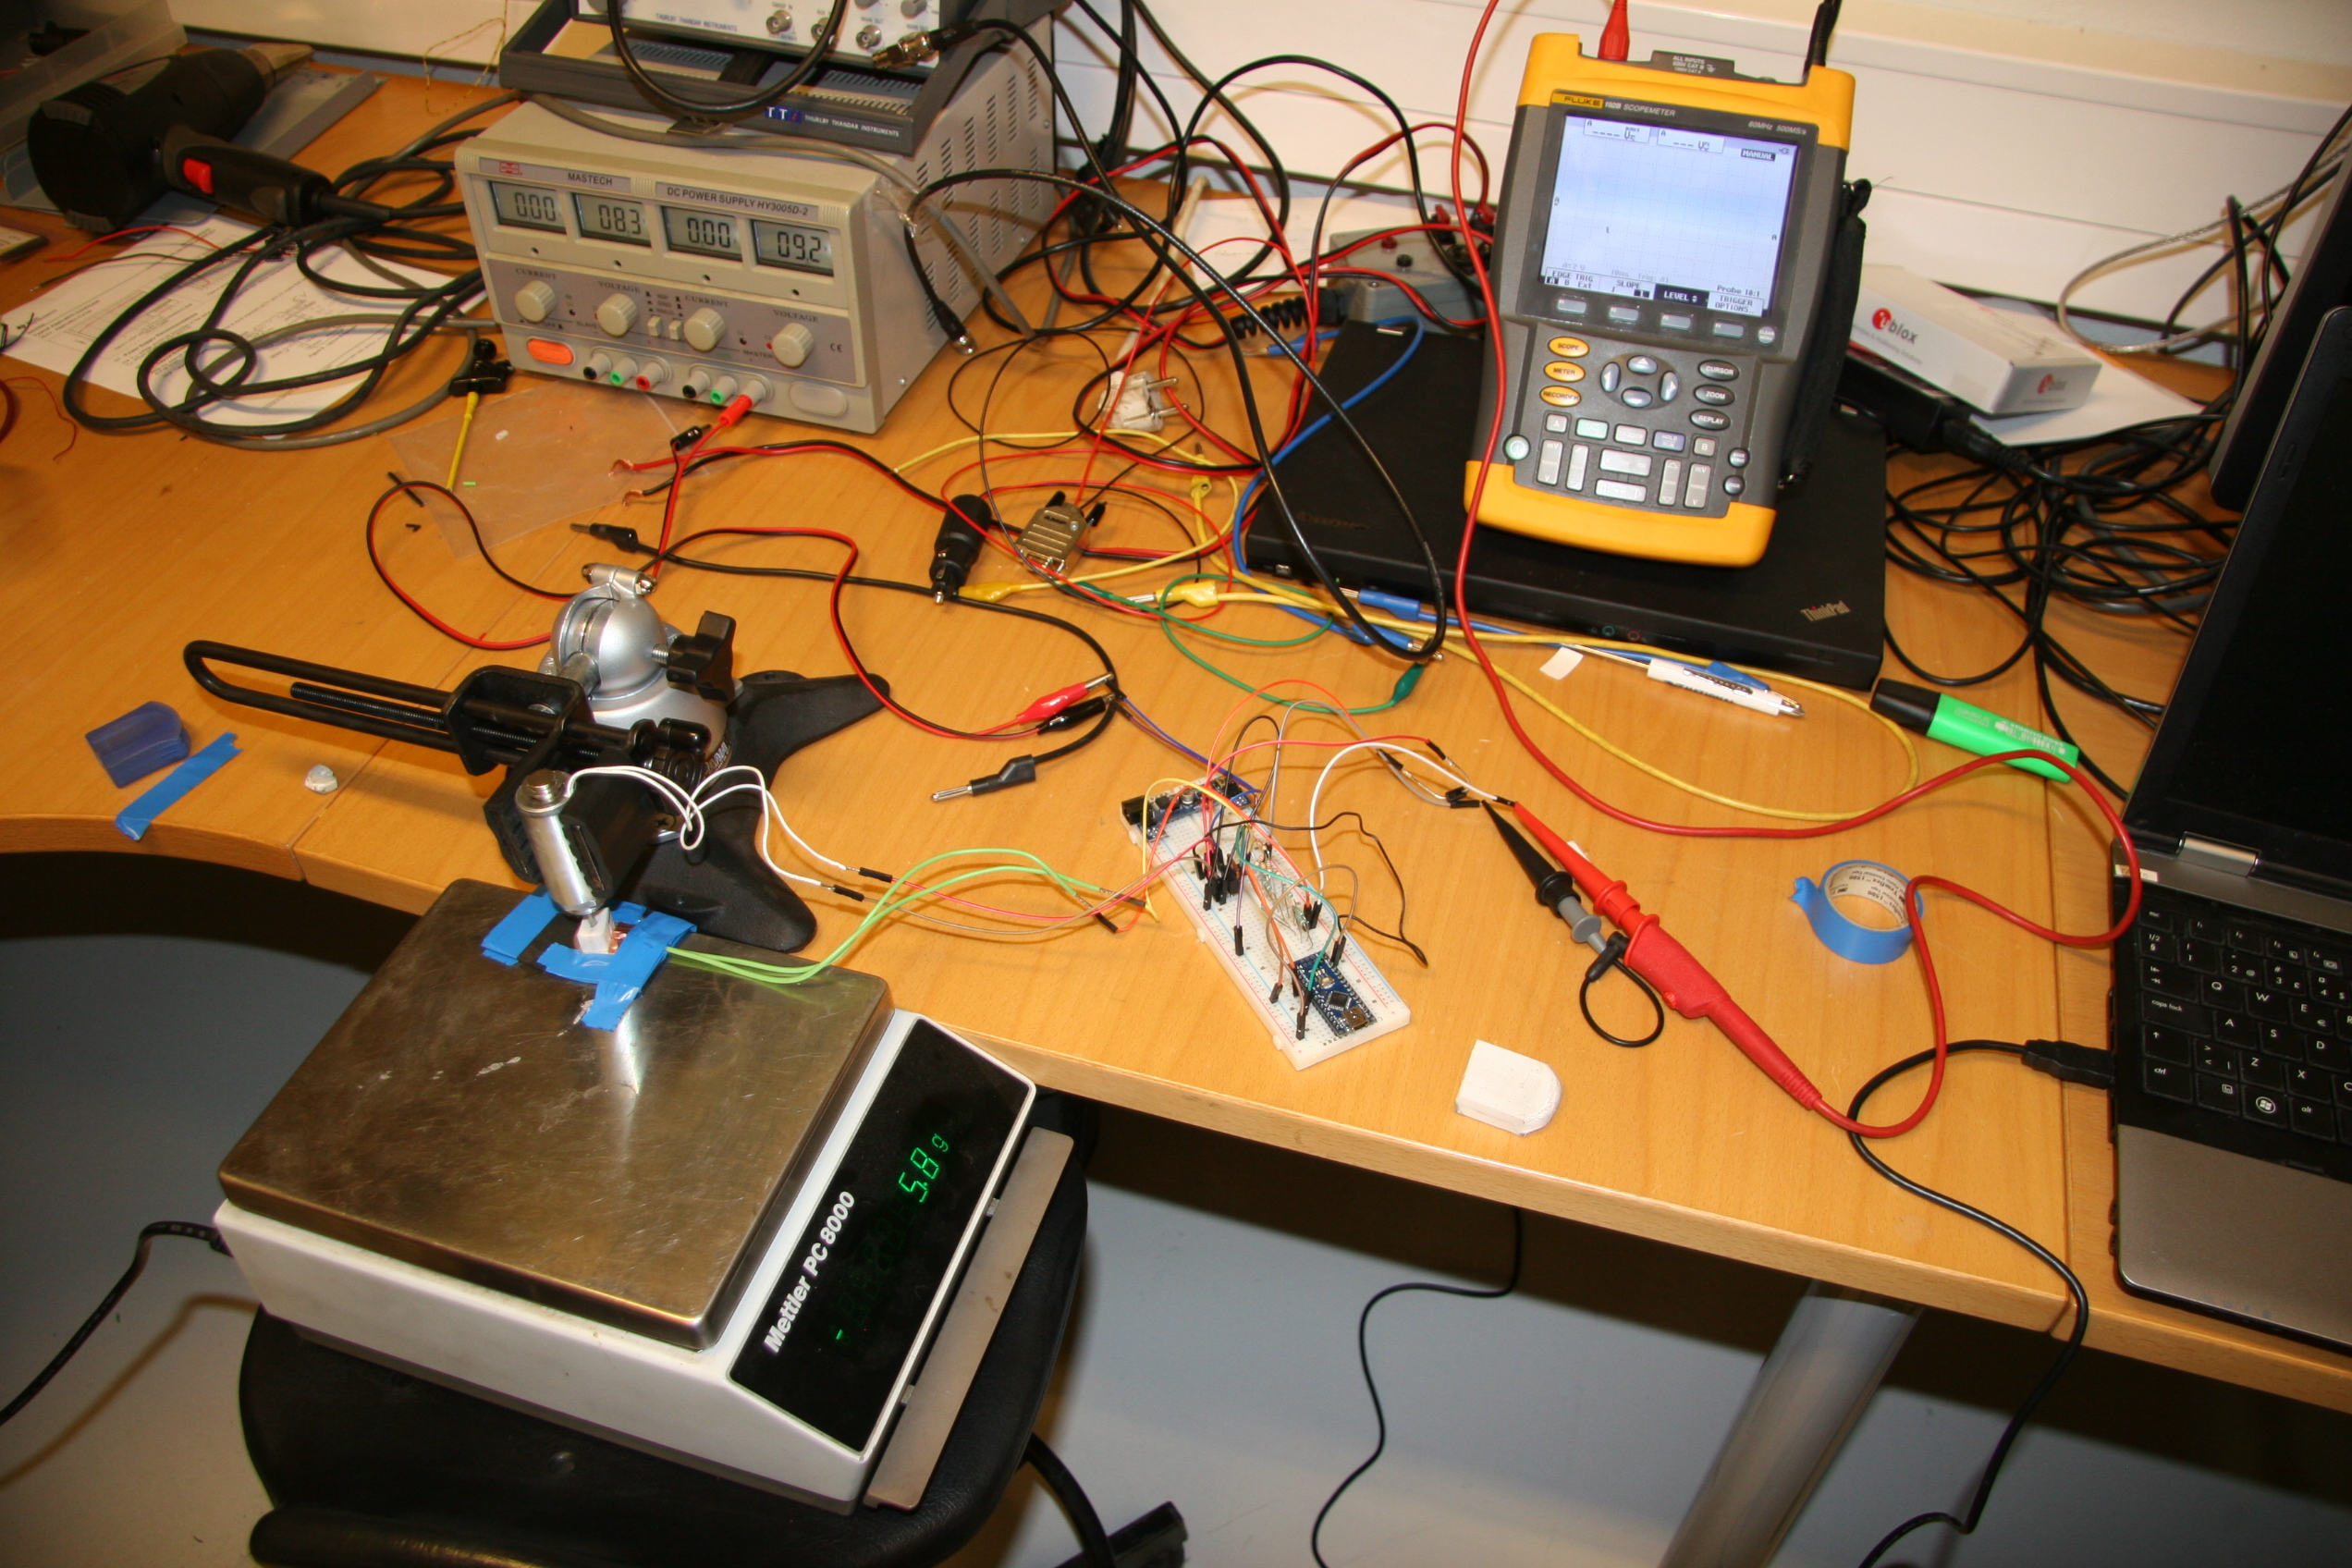
\includegraphics[height=6cm]{images/own_pic/piezo_test}
  \end{center}
  \caption{Test platform for piezo characteristics.}
  \label{fiq:piezo_impact}
\end{figure}

The measurement results are shown in figure \ref{fiq:piezo_measurement_chart}. Output voltage scales with square of impact force, which makes sense as work done can be expressed as $W = F * d$, where $W$ is work, $F$ is force and $d$ is distance force acts on object. As the displacement of piezo grows with the applied force, total work and therefore energy grows with both terms. 

\begin{figure}[htb]
  \begin{center}
  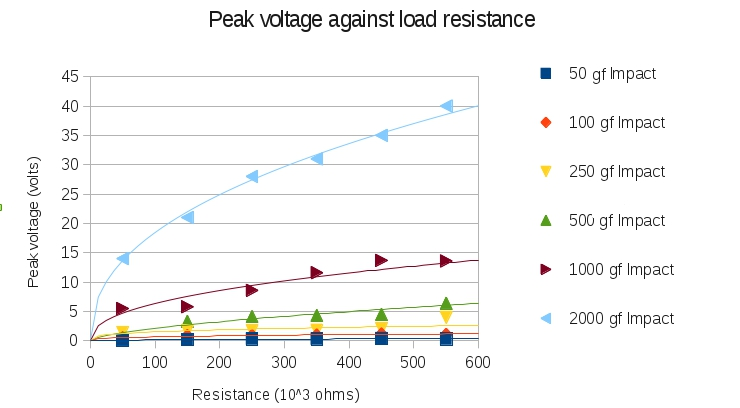
\includegraphics[height=6cm]{images/own_measurement/piezo_measurements}
  \end{center}
  \caption{Measured output voltage at different loads and impact forces.}
  \label{fiq:piezo_measurement_chart}
\end{figure}

Peak voltage grows with the load resistance. This makes sense in both voltage source and current source models, as the capacitor starts to discharge through load resistance instantly when voltage is applied over it. The relationship between voltage and load resistance seems to be logarithmic, which would be in good agreement with the logarithmic discharge curve of capacitor-resistor system. Peak voltages were read out from digital display and they can be considered reasonably accurate.

The time constants for voltage halving was graphically measured from oscilloscope waveforms, and this data was used to calculate the capacitance of TH-5C. These measurements are a lot less accurate, as readouts from oscilloscope screen have resolution of approximately half of line division, leaving accuracy of measurements at $\pm 2.5 ms$. These results are plotted in figure \ref{fig:piezo_time_capacitance}

\begin{figure}[htb]
  \begin{center}
  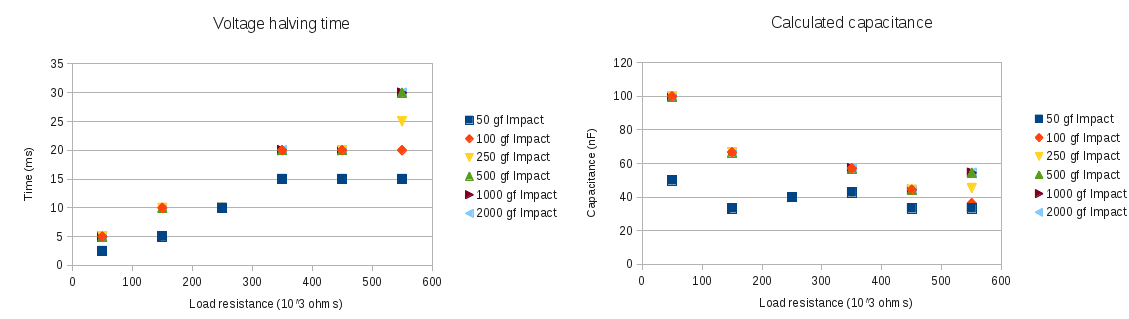
\includegraphics[height=4cm]{images/own_measurement/piezo_capacitance}
  \end{center}
  \caption{Measured half-time of system and calculated capacitance of piezo.}
  \label{fig:piezo_time_capacitance}
\end{figure}

The half-time data can be used to calculate capacitance of piezo using the RC-time constant of circuit:

\begin{equation}
  C=\frac{t}{-ln(\frac{1}{2})R} 
\end{equation}

 TH-5C provides value of 39nF as the capacitance, while these calculated values are notably higher and rise with the loading of piezo. Most likely explanation of this observation is the mechanical response time of system: solenoid plunger will take some milliseconds to reach new force equilibrium, and this effect becomes more pronounced at smaller time constants of RC-system. Using the known voltage and capacitance energy and peak power in impact can be determined:
 
\begin{equation}
   E = \frac{1}{2}V^2C
\end{equation}

\begin{equation}
   P_{peak} = \frac{V^2}{R}
\end{equation}
 
 The calculations are plotted in graph \ref{fig:piezo_power_energy}. As these calculations are based on inaccurately measured time, they should not be used as reference for any further calculations. However, trends can be seen in these values. 
 
 Interestingly the peak work done by piezo to resistor seems to be almost constant on all load levels. This is probably a consequence of logarithmic voltage-load relationship described above. There is a possibly significant result based on these findings: total energy obtainable from harvester grows with load resistance. However, this is applicable only for resistive load under impact-based energy generation.
 
 \begin{figure}[htb]
  \begin{center}
  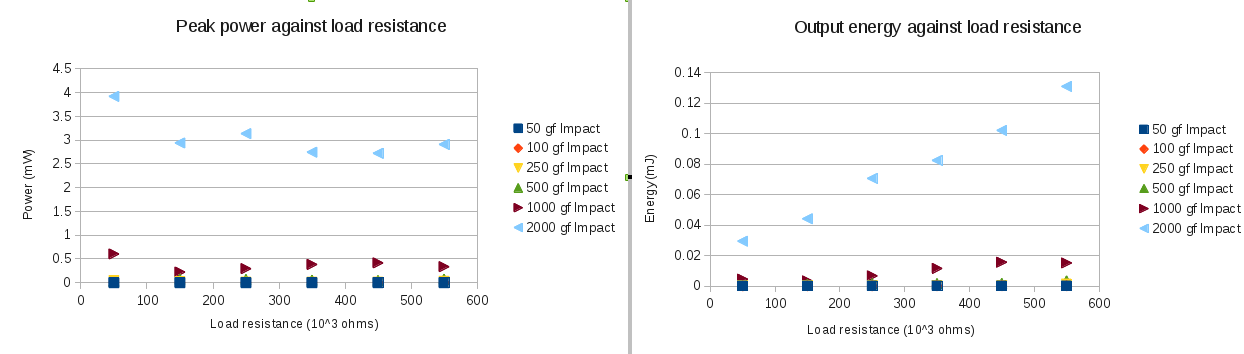
\includegraphics[height=4cm]{images/own_measurement/piezo_power}
  \end{center}
  \caption{Calculated piezo power and energy output}
  \label{fig:piezo_power_energy}
\end{figure}

Based on these results, an electrical equivalent model of circuit was designed. The model is shown in figure \ref{fig:piezo_ltspice_equivalent}. Model has two parallel current sources, one to simulate impact of plunger on piezo and other to simulate release of the impact. Capacitance in parallel is set to 39 nF as given in datasheet, load resistance is parametrised to step through the experimental values. 

Model was tuned by first calculating the total current transfer to reach the open circuit voltage over capacitor. Then maximum current of current sources was matched to reach peak voltage over highest load.
The simulated data is plotted figure \ref{fiq:piezo_simulation_experimental}.

 \begin{figure}[htb]
  \begin{center}
  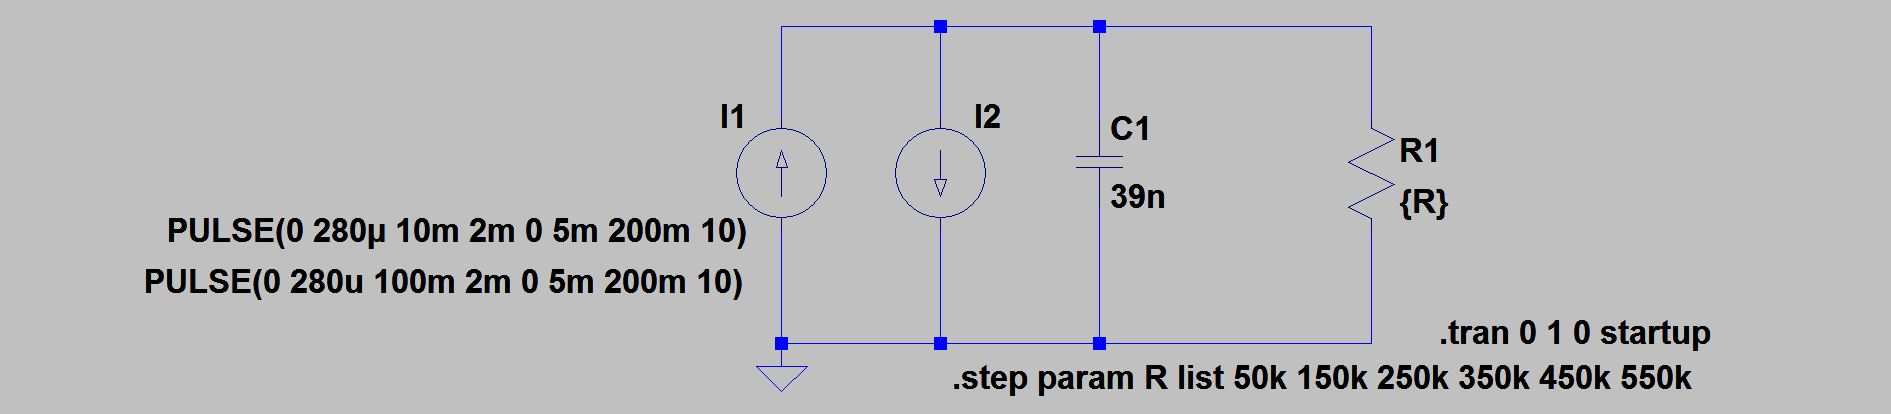
\includegraphics[height=6cm]{images/own_dwg/ltspice_piezo}
  \end{center}
  \caption{Equivalent model of piezo in LTSpice simulator}
  \label{fig:piezo_ltspice_equivalent}
\end{figure}

 \begin{figure}[htb]
  \begin{center}
  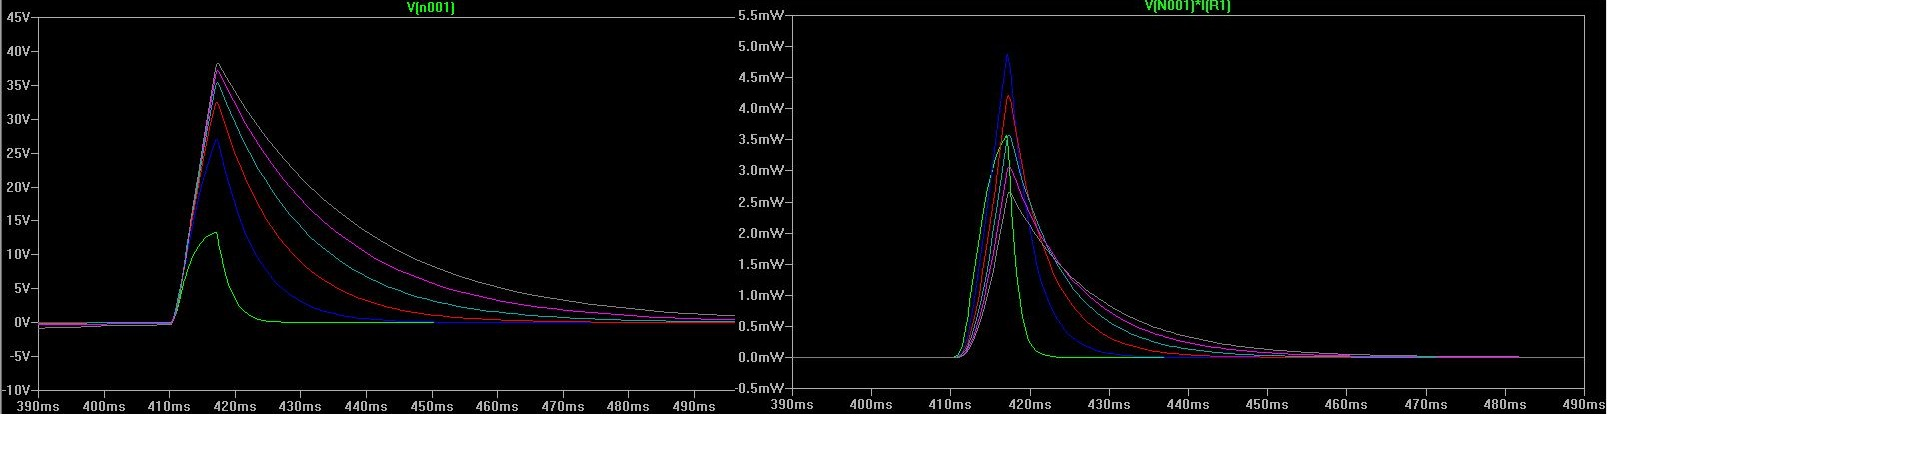
\includegraphics[height=8cm]{images/own_dwg/ltspice_piezo_simulation}
  \end{center}
  \caption{Simulated piezoelement output voltage and power waveforms. Loads are stepped through list to match experimental values at 2000 gf impact force. Black: 50k; Blue: 150k; Red: 250k; Turquoise: 350k; Violet: 450k; Gray: 550k}
  \label{fiq:piezo_simulation_experimental}
\end{figure}

The experimental and simulated data are not in a good agreement. While maximum and minimum load voltage and power are close to estimated values, this is by design as model is tuned to these measurements. Problems occur in interpolating the results, as output voltages are notably higher than measured values. This provides a result which sets the maximum power load near the value which provides output voltage of half of the open loop voltage. This is especially interesting as LTC3331 datasheet \cite{LTC3331} suggests to set the circuit to track the load at this same half-point of open loop voltage. Both LTC3331 and LTSpice are made by Linear Technology, so independent verification of this result would be needed. 

\subsection{Electronic design} \label{sect:electronic_design}
\subsubsection{Simulation of circuit}
As the focus of work is in energy harvesting, only analog sections related to energy harvesting are simulated. Digital loads are simulated as current sinks. This section details the simulation model used to validate the design of circuitry.

The analog sections of circuit were simulated using LTSpice IV \cite{ltspice}. Microcontroller, radiolink and accelerometer were simulated as resistive load. Battery was modelled as a voltage source with high-value capacitor and low-value resistor in series. Piezoelectric harvesting was modelled both as high-voltage source with capacitor in series and current source with capacitor in parallel. Electromagnetic harvesting was modelled as low-impedance low-voltage source. 

LTC3331 presents an interesting opportunity for maximum power point tracking (MPPT). While the impedances of individual components cannot be tuned in real-time, the microcontroller can determine rotation frequency of tyre from accelerometer readings and determine the maximum power point. LTC3331 can adjust the target voltage for energy storage buffer capacitor, which enables MPPT-control of system.

The simulation model is shown in figure \ref{fig:ltspice_sim}. Connections were adjusted as needed to generate simulation data for different purposes, such measuring energy efficiency, transient response, MPPT etc.

\begin{figure}[htb]
\begin{center}
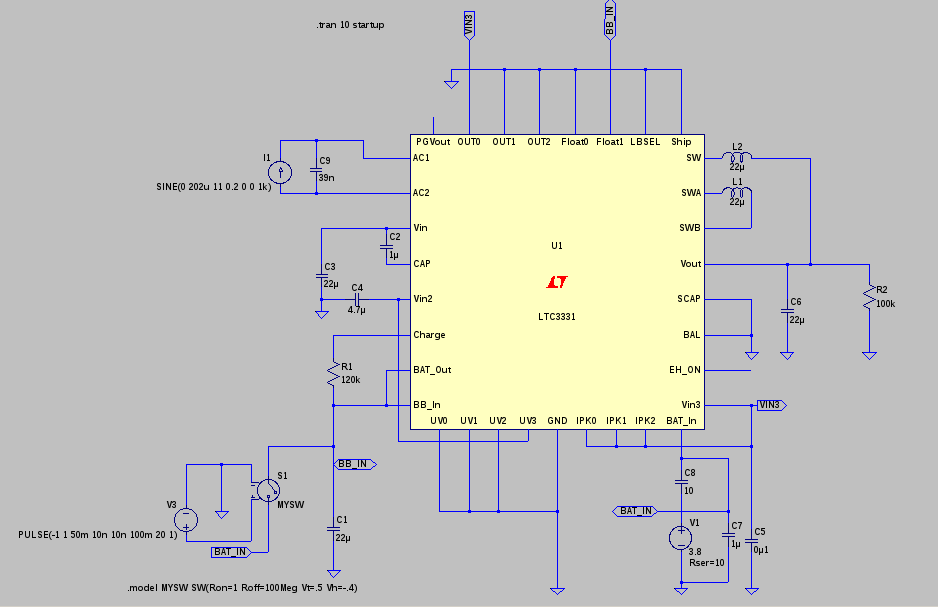
\includegraphics[height=12cm]{images/own_dwg/ltspice_ltc3331.jpg}
\end{center}
\caption{\label{fig:ltspice_sim} LTSpice \cite{ltspice} simulation of electrical circuit}
\end{figure}

The simulation model was used to validate basic operation of circuit. Circuit operates as datasheet specified. MPPT algorithms can be developed after the experimental results from energy harvesting are obtained. 

As the basic operation of circuit has been validated, next step is to design the detailed schematic for the circuit. The next section details schematic design of the circuit, starting from top-level diagram and connections between blocks, followed by detailed design of each subblock. 

\subsubsection{Schematic design}
The printed circuit board (PCB) schematic is a logical representation of the components and how they connect to each other. The schematic is designed in accordance to datasheets, reference designs and application notes of main circuit components. This section details the schematic diagram of the circuit.

As the design operates in high-vibration environment with wide temperature variations, special care is used to select components which have well-defined temperature and mechanical characteristics. 

As the circuit is a low-power design, careful attention has to be paid to parasitic properties and non-ideal behaviour of components. For example electrolytic capacitor can have leakage current of several microamperes \cite{Both2001}, which is in the same order of magnitude as the targeted sleep current consumption of system. Likewise any signalling current should be kept at minimum. 

Another important point of view is the modularity and testability of the circuit. All critical lines have provision for testing and debugging for development and verification of circuit functionality. Figure \ref{fig:circuit_blocklevel} shows the interconnections in system, drawn in KiCAD \cite{KiCAD}.  The power supply can be cut off to separate sections of circuit for current measurement as needed. This has additional benefit of leaving places for power supply filtering components in case some section of circuit emits electrical noise through power supply lines.

\begin{figure}
    \centering
    \def\svgwidth{\columnwidth}
    \input{images/own_dwg/circuit/radio.pdf_tex}
    \caption{\label{fig:circuit_blocklevel} System level design of electronics}
\end{figure}

Power supply has some conflicting requirements, as any noise in power degrades radio and measurement performance, but on the other hand the power supply should be efficient switch mode power supply to keep power consumption at minimum. LTC3331 has switch-mode power supplies which can be used to generate supply rails for the rest of circuit, these are used and noise is dealt with by passive filtering. Most of the power supply design \ref{fig:psu_circuit} is relatively straightforward application of ideas presented in LTC3331 datasheet, but a few special considerations have been given to tailor the power supply for application. Device is configurable by soldering appropriate resistors, and the energy harvesting MPPT can be controlled by external microcontroller using signals UV[0:3]. 

Battery configuration allows different chemistries to be tested, as the under- and overvoltage lockout levels are user selectable. If a non-rechargeable battery is desired, battery charging can be disabled by omitting resistor R201. 

\begin{figure}
    \centering
    \def\svgwidth{\columnwidth}
    \input{images/own_dwg/circuit/harvester.pdf_tex}
    \caption{\label{fig:psu_circuit} Power supply with harvesting input, battery management and SMPS voltage output.}
\end{figure}

Central controller is built around ATMEGA328 \cite{atmega328} microcontroller. The controller uses SPI and UART serial communication between sections of the system, and it has parallel connection to LTC3331 to set the energy harvester voltage levels for MPPT. LTC3331 has EH\_ON output, which rises to logic high level of approximately 4.8 volts when the circuit is being supplied by harvested energy rahter than by a battery. This voltage level is above the circuit supply voltage, and therefore interfacing it directly to ATMEGA328 would be damaging. Interfacing is done by N-MOSFET BSH105 \cite{BSH105} and internal pullup-resistor on ATMEGA328. When harvested energy is available, pull-up of ATMEGA328 becomes grounded through BSH105. This causes somewhat significant current leakage, in range of tens of microamperes while pull-up is being pulled down. However this leakage is present only while harvested energy is available, so it will not drain the battery of circuit. While harvested energy is not available, the MOSFET is shut off. Special care was taken to select a model of MOSFET with small off leakage to avoid drain while system is being run on battery power, BSH105 is specified to have leakage in range of tens of nanoamperes. 

Most important power saving is achieved through careful design of software. Sleep power states of ATMEGA328 consume miniscule amount of power when compared to active state, therefore minimizing active time of circuit is a high priority. If the program is not CPU time limited, clock rate can be scaled down to 1 MHz using internal clock divider. Maximum CPU frequency can be incresed by selecting another crystal, but increasing clock frequency will require higher supply voltage which in turn leads to higher overall power consumption in entire system.

\begin{figure}
    \centering
    \def\svgwidth{\columnwidth}
    \input{images/own_dwg/circuit/control.pdf_tex}
    \caption{\label{fig:atmega_circuit} Control circuit with external interrupts from sensor and energy harvesting.}
\end{figure}

Radio link is implemented with BLE113 module. The module could act as stand-alone controller for the system, but radio link has been separated from control logic to allow focused study of different sections of circuit.  Schematic  \ref{fig:bluetooth_circuit} is very simple, power supply is decoupled by bypassing capacitors as recommended by datasheet and programming header has been brought out. Communication to microcontroller is handled by universal asynchronous receiver/transmitter (UART) communication using 2.5 V level signaling. 

BLE113 can be forced to sleep by external control if needed and it can operate autonomously while main controller is sleeping. Data payload can be up to 20 bytes per packet as specified by BLE protocol {\color{red}cite}, maximum data throughput is defined by connection interval. As transmitting data consumes active time and therefore power, data transmissions should be minimized while harvested energy is not available.

\begin{figure}
    \centering
    \def\svgwidth{\columnwidth}
    \input{images/own_dwg/circuit/bluetooth.pdf_tex}
    \caption{\label{fig:bluetooth_circuit} Bluetooth connectivity built with BLE113 module}
\end{figure}

There is an accelometer ADXL375 onboard the PCB to study applications of tyre sensor system. Schematic of sensor section is shown in figure \ref{fig:sensor_circuit}. The power supply section has a separate digital Input/Output (IO) supply voltage which is further filtered for analog sections of board by FB501 and C502. Both supplies are fed by same system level power bus from LTC3331.

ADXL375 is capable of both SPI and I2C communication, SPI communication was selected to facilitate faster communication to minimize time control circuit has to be in awake and to avoid additional power drain through the required pull-up resistors of I2C bus. On the other hand, the circuit has a design feature which requires usage of OR gate to avoid SPI sequence being interpreted as I2C command. The OR was selected to be SN74AUP1T32 \cite{orgate}, which has minimal static power current consumption of 0.1 microamperes. 

\begin{figure}
    \centering
    \def\svgwidth{\columnwidth}
    \input{images/own_dwg/circuit/sensor.pdf_tex}
    \caption{\label{fig:sensor_circuit} Accelerometer circuit}
\end{figure}

As the circuit will be subject to extreme accelerations, all the components should be surface mounted. This gives maximal solder pad area to height ratios, which helps to maintain the integrity of circuit. Larger components, such as inductors can be additionally glued for increased mechanical reliability.

The estimated current draw for each of the subcircuits dominated by the main integrated circuit of each subcircuit. The power consumption estimates were presented in section \ref{sect:power_requirement} table \ref{power_consumption_table}.

As the schematic was finished, next task was to design the layout of the circuit. Next section describes the design process of laying out the circuit and shows the completed design of circuit board.

\subsubsection{Circuit layout}
The PCB layout defines the physical placement of the components on the circuit board. Process of laying out the circuit as well as the structure of printed circuit board is described in this section.

Usually circuits are laid out by defining the outline of the board. Then any mechanical constraints, such as mounting holes and connectors are placed. Next step is to place the main ICs. As the main features of circuit are defined, subsections of circuit is planned. Critical and sensitive components such as crystals and antennas are placed as first priority. Then the power supply lines and power supply components are placed, in this case the inductors and capacitors of SMPS are placed as close as possible to relevant pins. 

As the design operates in high-vibration environment with wide temperature variations, special care is used to select components which have well-defined temperature and mechanical characteristics.

The circuit is laid out on 4-layer PCB, where inner layers are dedicated to ground and power planes. This means that power supply decoupling needs a lot less care than on 2-layer board, generally a via straight from power pin to relevant plane gives low-impedance supply to circuit. Power supply decoupling capacitors are still placed as close as possible to relevant pins and power supply pins are fed directly from capacitors when possible to minimize power supply noise leaking into power planes.

Finally the rest of the circuit is laid out. As the currents flowing on board are relatively small and signal rates are low, routing can be rather carefree on non-critical sections. Final board is shown in figure \ref{fig:pcb_render}. Energy harvesting section is at left, radio is on top, control section is at right and accelerometer is at bottom. 

\begin{figure}[htb]
  \begin{center}
    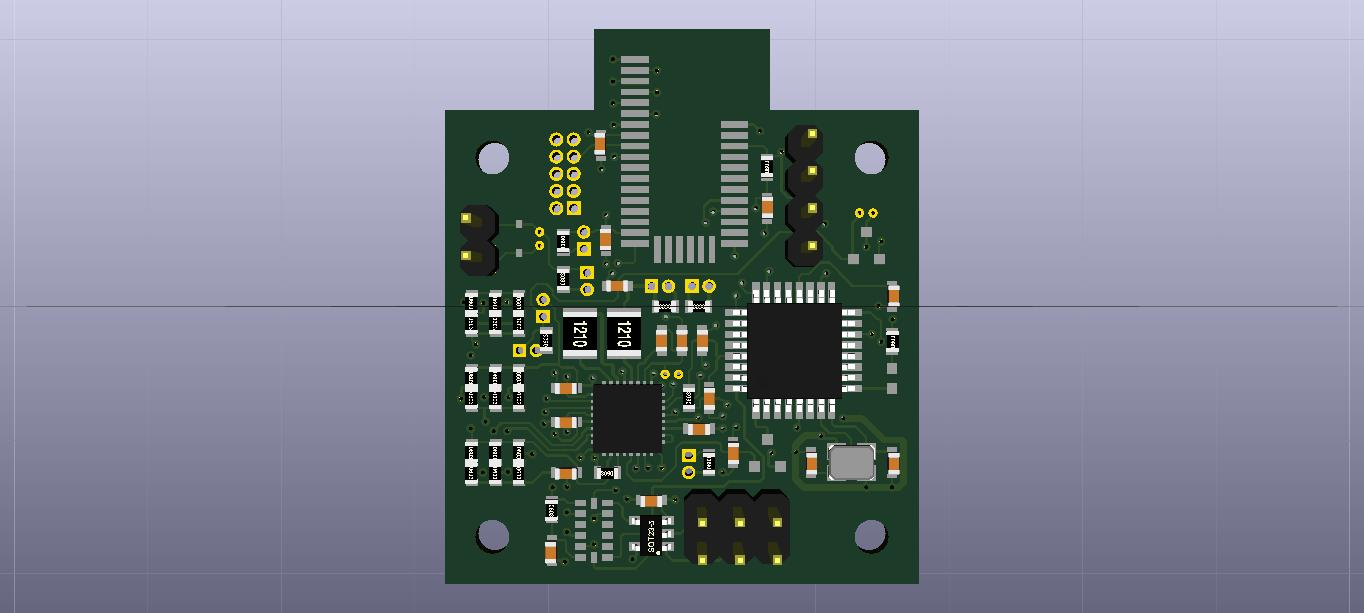
\includegraphics[height=6cm]{images/own_dwg/circuit/render.jpg}
  \end{center}
  \caption{\label{fig:pcb_render} Render of the final PCB}
\end{figure}

The borders between sections are most clearly visible in the power planes of design shown in figure \ref{fig:pcb_planes}. Power planes for each subcircuit have been separated for testing the current consumption, and therefore the outlines of power planes follow the outlines of subcircuits.

\begin{figure}[htb]
  \begin{center}
    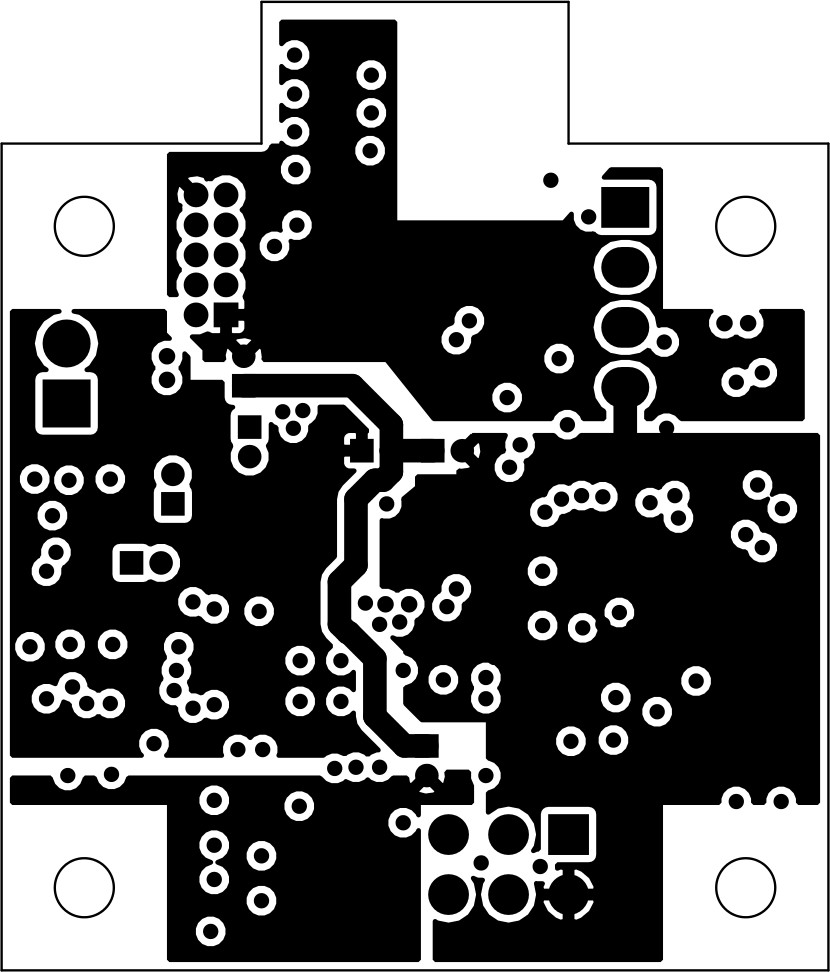
\includegraphics[height=6cm]{images/own_dwg/circuit/powerplane.jpg}
  \end{center}
  \caption{\label{fig:pcb_planes} Power planes of the PCB}
\end{figure}

In addition to mechanical and electrical properties, the PCB also acts as heat sink for mid-power components. In this circuit only LTC3331 needs special attention to thermal design, it is cooled by several vias under the pad of circuit into ground plane. As copper is excellent conductor for heat, any thermal output from LTC3331 gets coupled to groundplane where it can spread to a wider area.

Battery holder is only large component in design where G-forces might cause a problem. The holder is on the backside of the pcb, where it can be mounted using adhesives or it can be supported by harvester top.

\subsection{Mechanical design of harvester}
This section details the mechanical considerations for both harvester types. First material options are explored, then the design for generators is presented.

Material for the generator has a few requirements. It has to have at least as good temperature characteristics as the magnet being used and it must be hard enough to not deform under impacts. Low friction coefficient is desirable as this leads to smaller losses, and long time durability under wear is of course desired. Being lightweight and easily machinable are also desired characteristics. As the generator is small, volumetric cost of the material is of little concern. For the electro-magnetic generator design material ferromagnetism has to be considered. Table \ref{parameters_of_materials} has comparison of different materials considered for the application.

\begin{table}[htb]
%% Taulukon teksti
\caption{\label{parameters_of_materials} Materials for the shaft of generator \cite{PlasticsInternational2015}, \cite{Etra}, \cite{Goodfellow} \cite{McCarr}.}
\begin{center}
\fbox{
\begin{tabular}{l l l l l l}
\textbf{Material}& 
\textbf{Hardness}& 
\textbf{Friction} & 
\textbf{Durability} & 
\textbf{Temperature}\\ \hline
PTFE(Teflon)      & Very low   & Lowest                      & Lowest    & -190... + 250 \degree C \\ \hline
Polycarbonate     & Very high  & High       & -         & -60... + 125 \degree C \\ \hline
PA 6 (Nylon)      & Low        & Medium                      & High      & -40... + 80 \degree C  \\ \hline
Oil-infused Nylon & Low        & Very low                    & Very high & -20... + 105 \degree C \\ \hline
Acryllic          & High       & -                           & -         & -40... + 70 \degree C \\ \hline
Polyacetal (POM C)& Medium     & Low                         & Low       & -50... + 105 \degree C \\ \hline
Carbon fiber     & Highest     & Highest                         & High       & ... + 80 \degree C \\ \hline
\end{tabular}
}

\end{center}
\end{table}

There is no single best material for the harvester. Polycarbonate and carbon fibre would have excellent mechanical strength but they have high friction. Teflon and nylon would have lower friction, but they have poor mechanical rigidity. 

In the end Acryllic was chosen as the material of the harvester. While Acryllic is not a best material by any single metric, it has the necessary properties. Wide availability and ease of machining were decisive factors for the selection of acryllic over other materials. 

As the minimum diameter of harvester is defined by piezo element diameter of 34 mm, both generators are designed with 35 mm square bases. Both generators also use same mounting hole pattern for electronics - 2.75 mm holes at the corners of square.

Generator was machined using slices of laser cut acryllic and standard acryllic tubing. The process is somewhat similar to 3D-printing, as several thin layers form up the final part. The acryllic parts used in generator are shown in figure \ref{fig:lasercut}.

\begin{figure}[htb]
  \begin{center}
    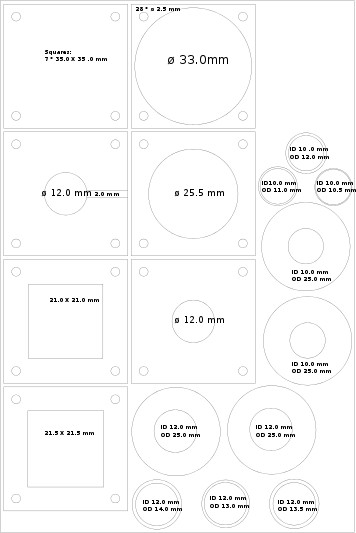
\includegraphics[height=15cm]{images/own_dwg/mechanical/layers.jpg}
  \end{center}
  \caption{\label{fig:lasercut} 150 * 150 mm sheet for laser cut.}
\end{figure}

While the initial approach for building the shaft of the generator was to use lasercut rings to form the shaft, the process of lasercutting warped thinner rings and mechanical alingment of the rings was difficult. Therefore a standard 10 mm inner diameter 12 mm outer diameter tube was selected as the shaft.

This section detailed the material options for the harvester structure and presented the manufacturing method. Acryllic was chosen as a compromise between material properties and availability for the generator. 

